\documentclass{beamer}

\usepackage[utf8]{inputenc}
\usepackage[T1]{fontenc}
\usepackage[english]{babel}
\usepackage{lmodern}
\usepackage{algorithm}
\usepackage{algorithmic}
\usepackage{mathtools}
\usepackage{hyperref}
\usepackage{multimedia}

\usetheme{UOS}

\graphicspath{{images/}}

\renewcommand{\baselinestretch}{1.25}

\begin{document}

\title{Normal Calculation in Point Clouds with CUDA}
\author[Matthias Greshake, Alexander Mock]{Alexander Mock, Matthias Greshake\\ {\scriptsize amock@uos.de, mgreshake@uos.de}}
\institute{Institut für Informatik\\ AG Wissensbasierte Systeme}
\date{26. January 2016}

\begin{frame}[plain]
	\titlepage
\end{frame}

\begin{frame}{Outline}
	\tableofcontents
\end{frame}

\section{Motivation}

\begin{frame}{Motivation}
	\centering
	\movie[width=11cm,height=6.1875cm,poster,autostart,loop]{}{Videos/kirche.mov}
\end{frame}

\begin{frame}{Point Clouds}
	\begin{columns}
		\begin{column}{0.5\textwidth}
			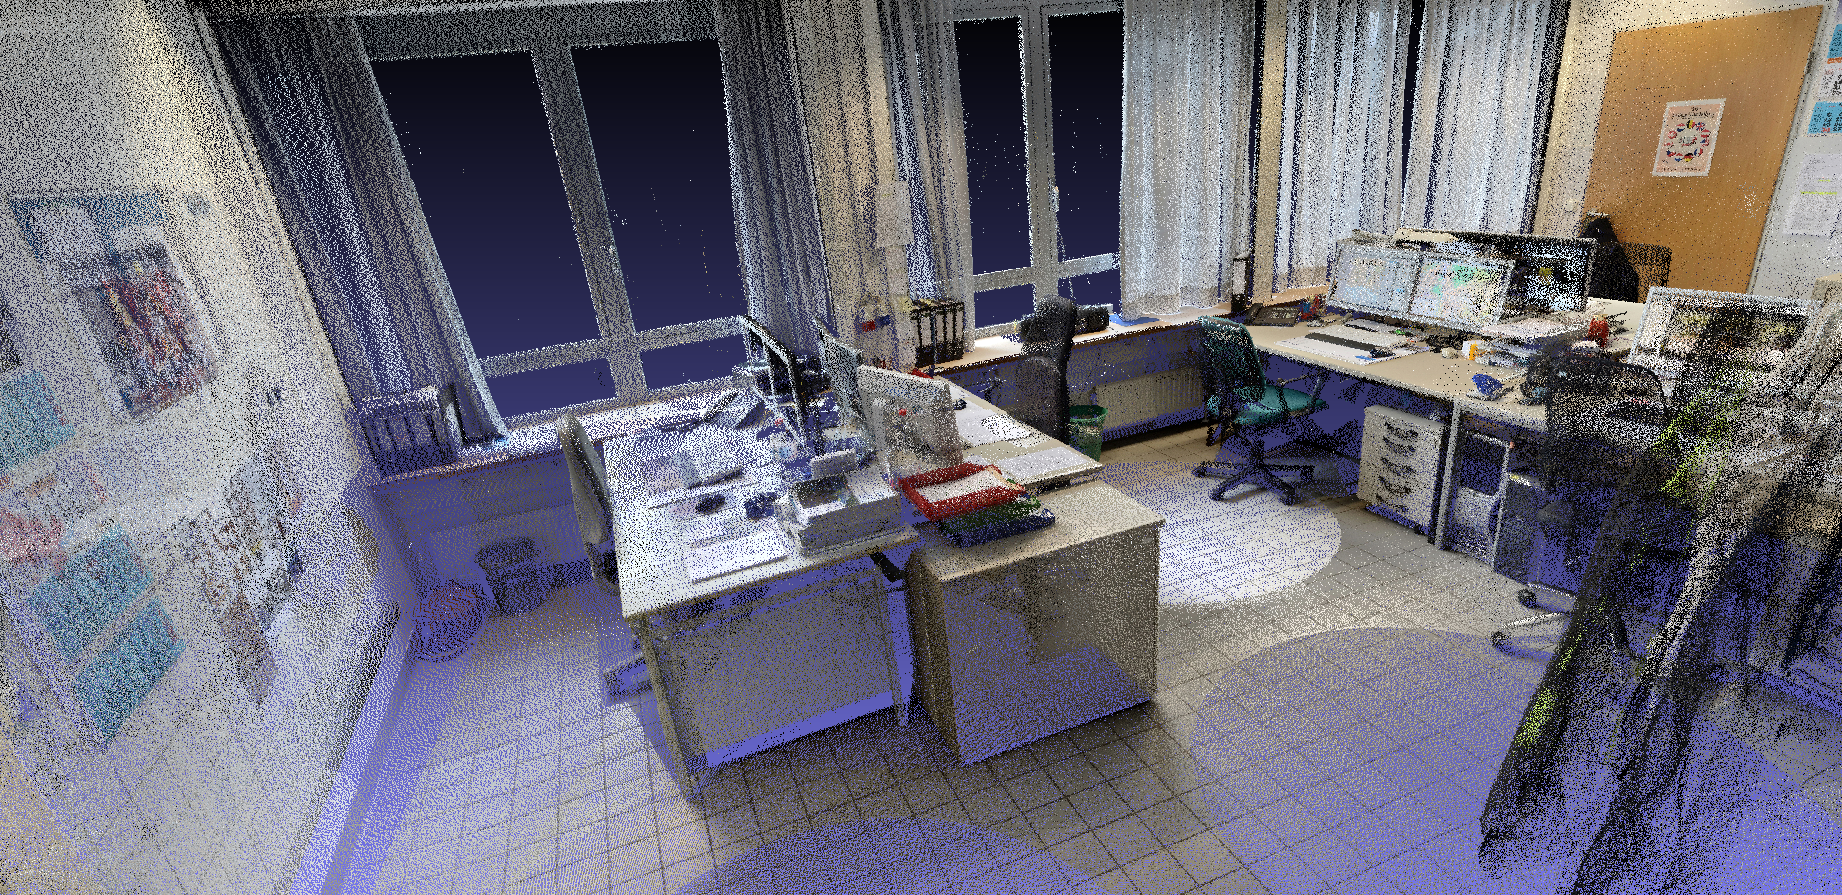
\includegraphics[width=1.0\textwidth]{point_cloud_1.png}\\
			\vspace{0.1cm}
			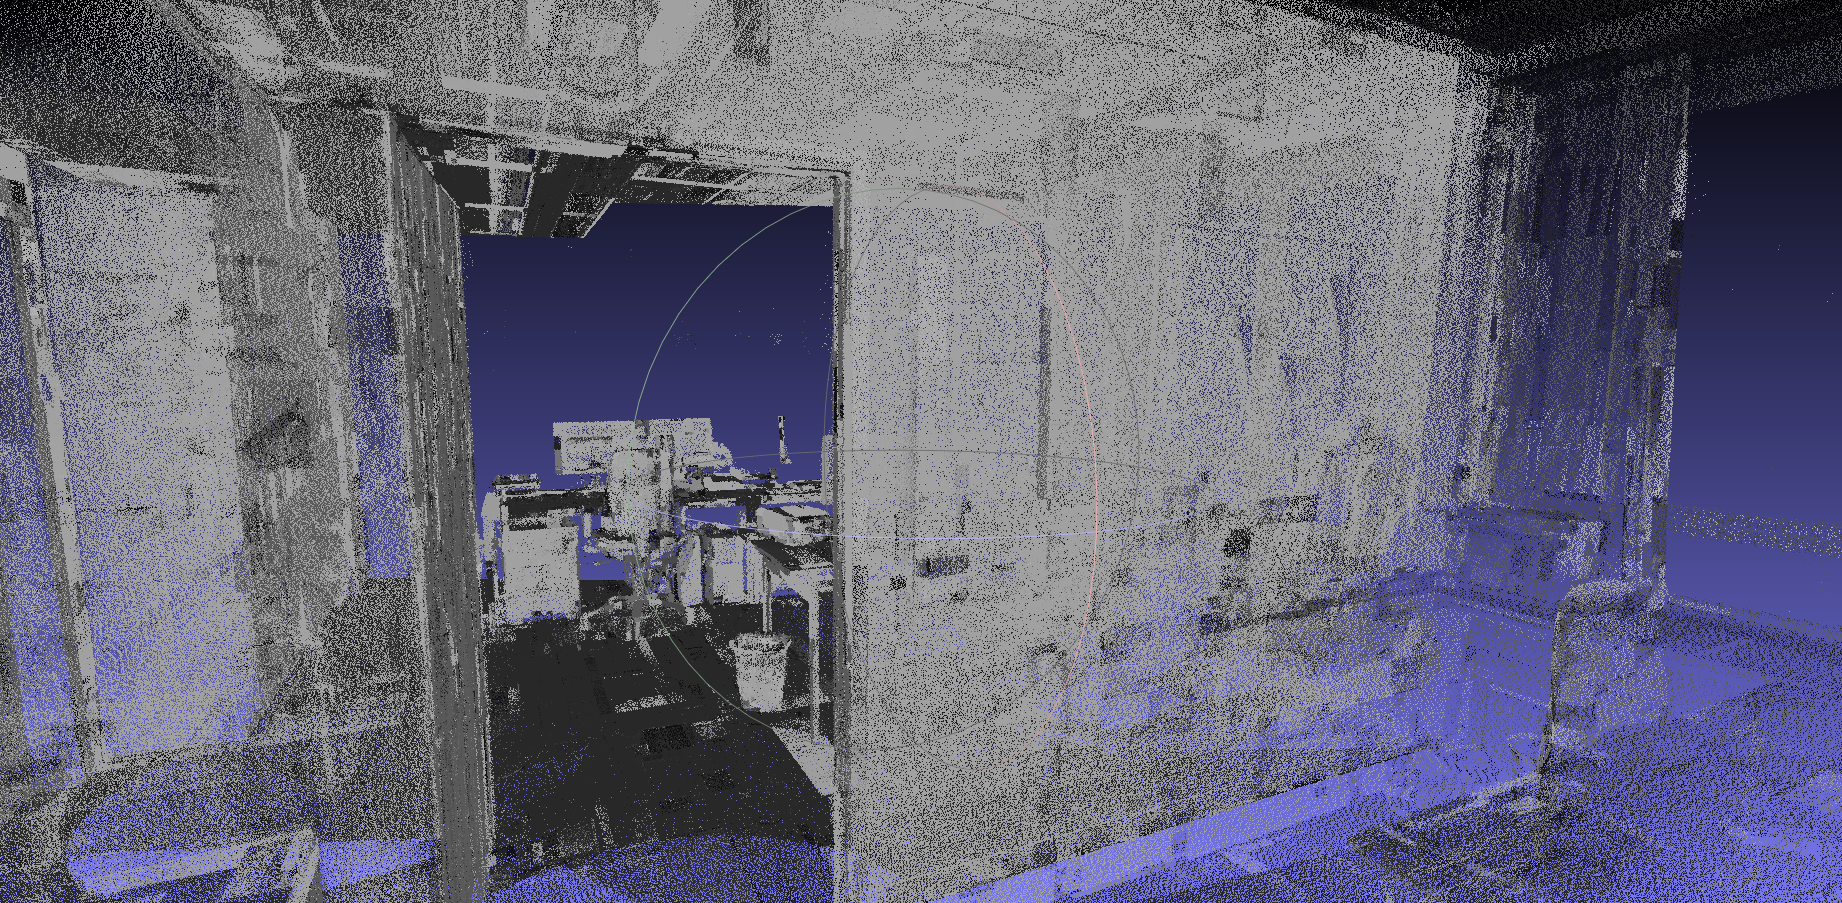
\includegraphics[width=1.0\textwidth]{police_point_cloud.png}
		\end{column}
		\begin{column}{0.5\textwidth}
			\begin{itemize}
				\item Generated by depth sensors of 3D laser scanners
				\item 3D points with geometry data of the environment
				\item No topological connection between points
				\item Polygonal meshes based on point clouds
			\end{itemize}
		\end{column}
	\end{columns}
\end{frame}

\begin{frame}{Reconstruction}
	\begin{columns}
		\begin{column}{0.5\textwidth}
			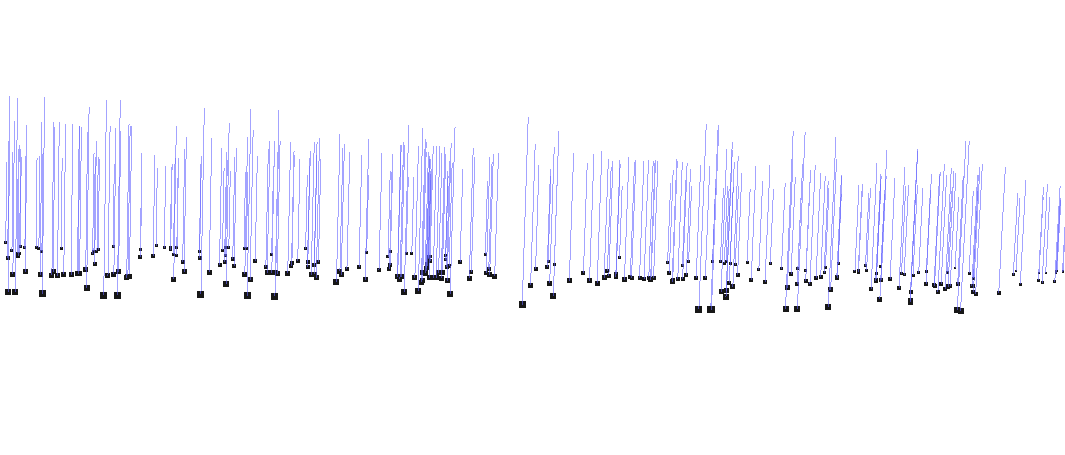
\includegraphics[width=1.0\textwidth]{normals.png}
			\vspace{0.1cm}
			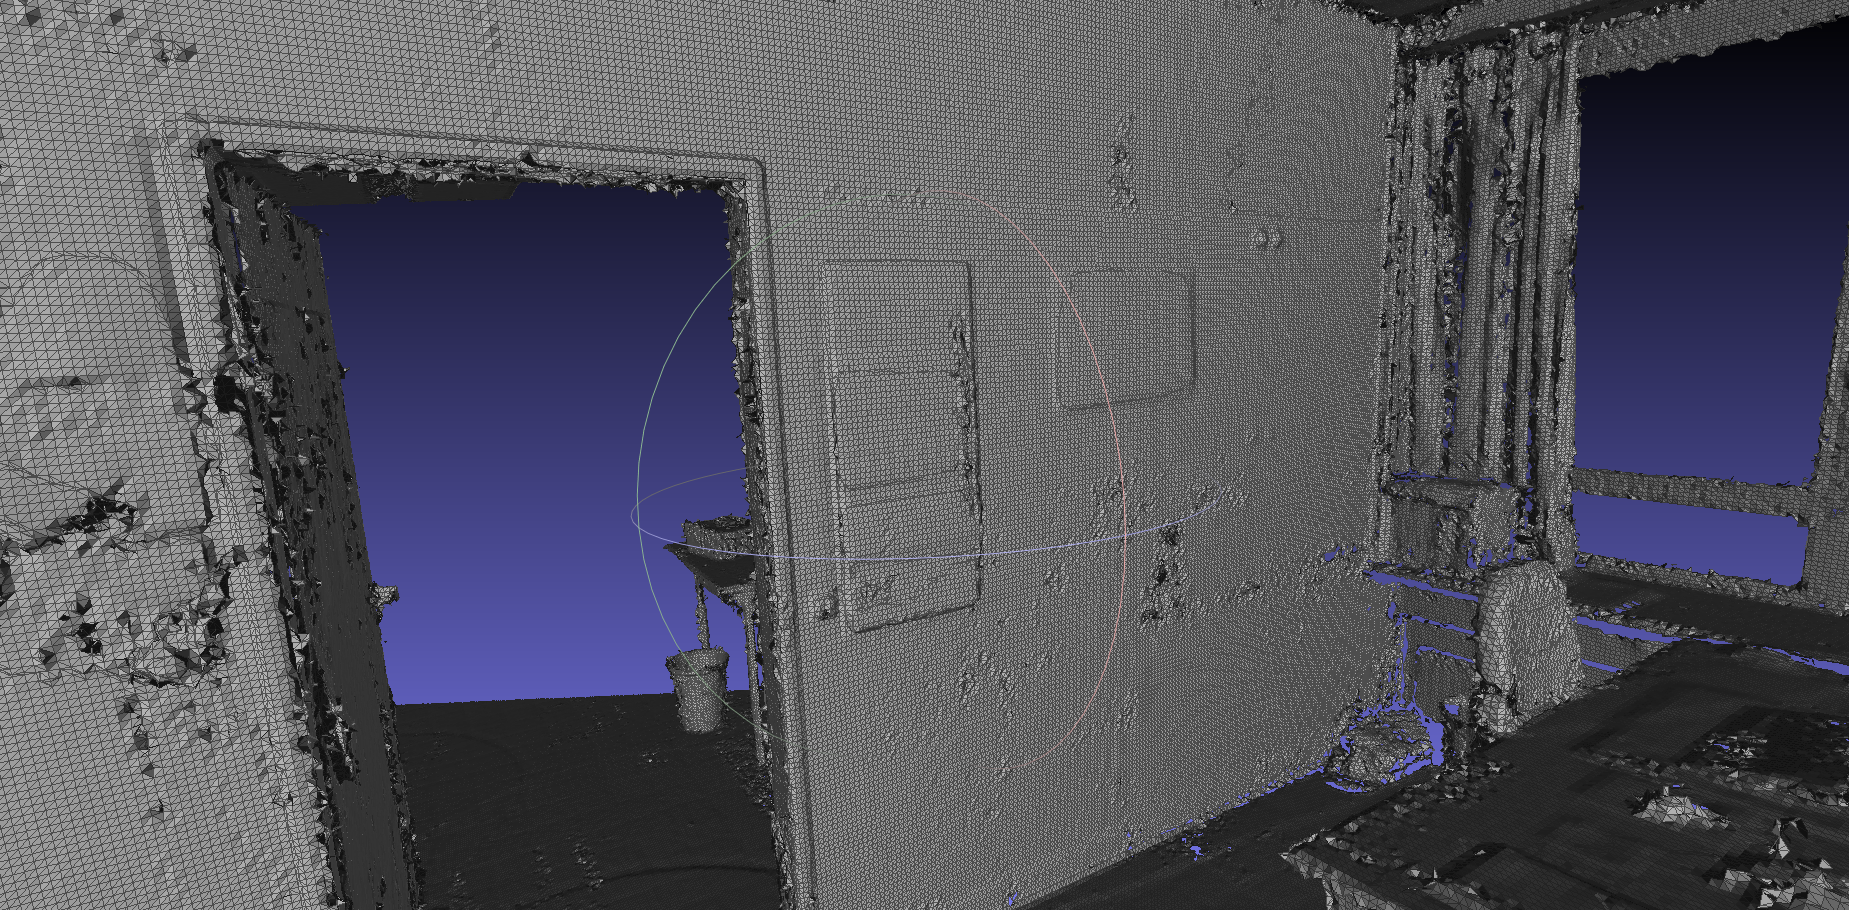
\includegraphics[width=1.0\textwidth]{police_mesh.png}
		\end{column}
		\begin{column}{0.5\textwidth}
			\begin{itemize}
				\item Lower memory usage without loss of information
				\item Normal of each point is necessary to create mesh
				\item Pre-calculation of normals is possible
				\item Requires nearest neighbours of each point
			\end{itemize}
		\end{column}
	\end{columns}
\end{frame}

\section{Problem Statement}

\begin{frame}{Nearest Neighbor Search}
	\begin{itemize}
		\item Independent search of k nearest neighbors to each point
		\item Long runtimes on large datasets
		\begin{block}{}
			\centering Nearest neighbor search is the bottleneck of normal calculation
		\end{block}
		\item Thread-based CPU implementation in the LVR Framework
	\end{itemize}
	\medskip
	\centering $\Rightarrow$ Parallel implementation on GPU to reduce runtime
\end{frame}

\begin{frame}{GPU vs. CPU}
	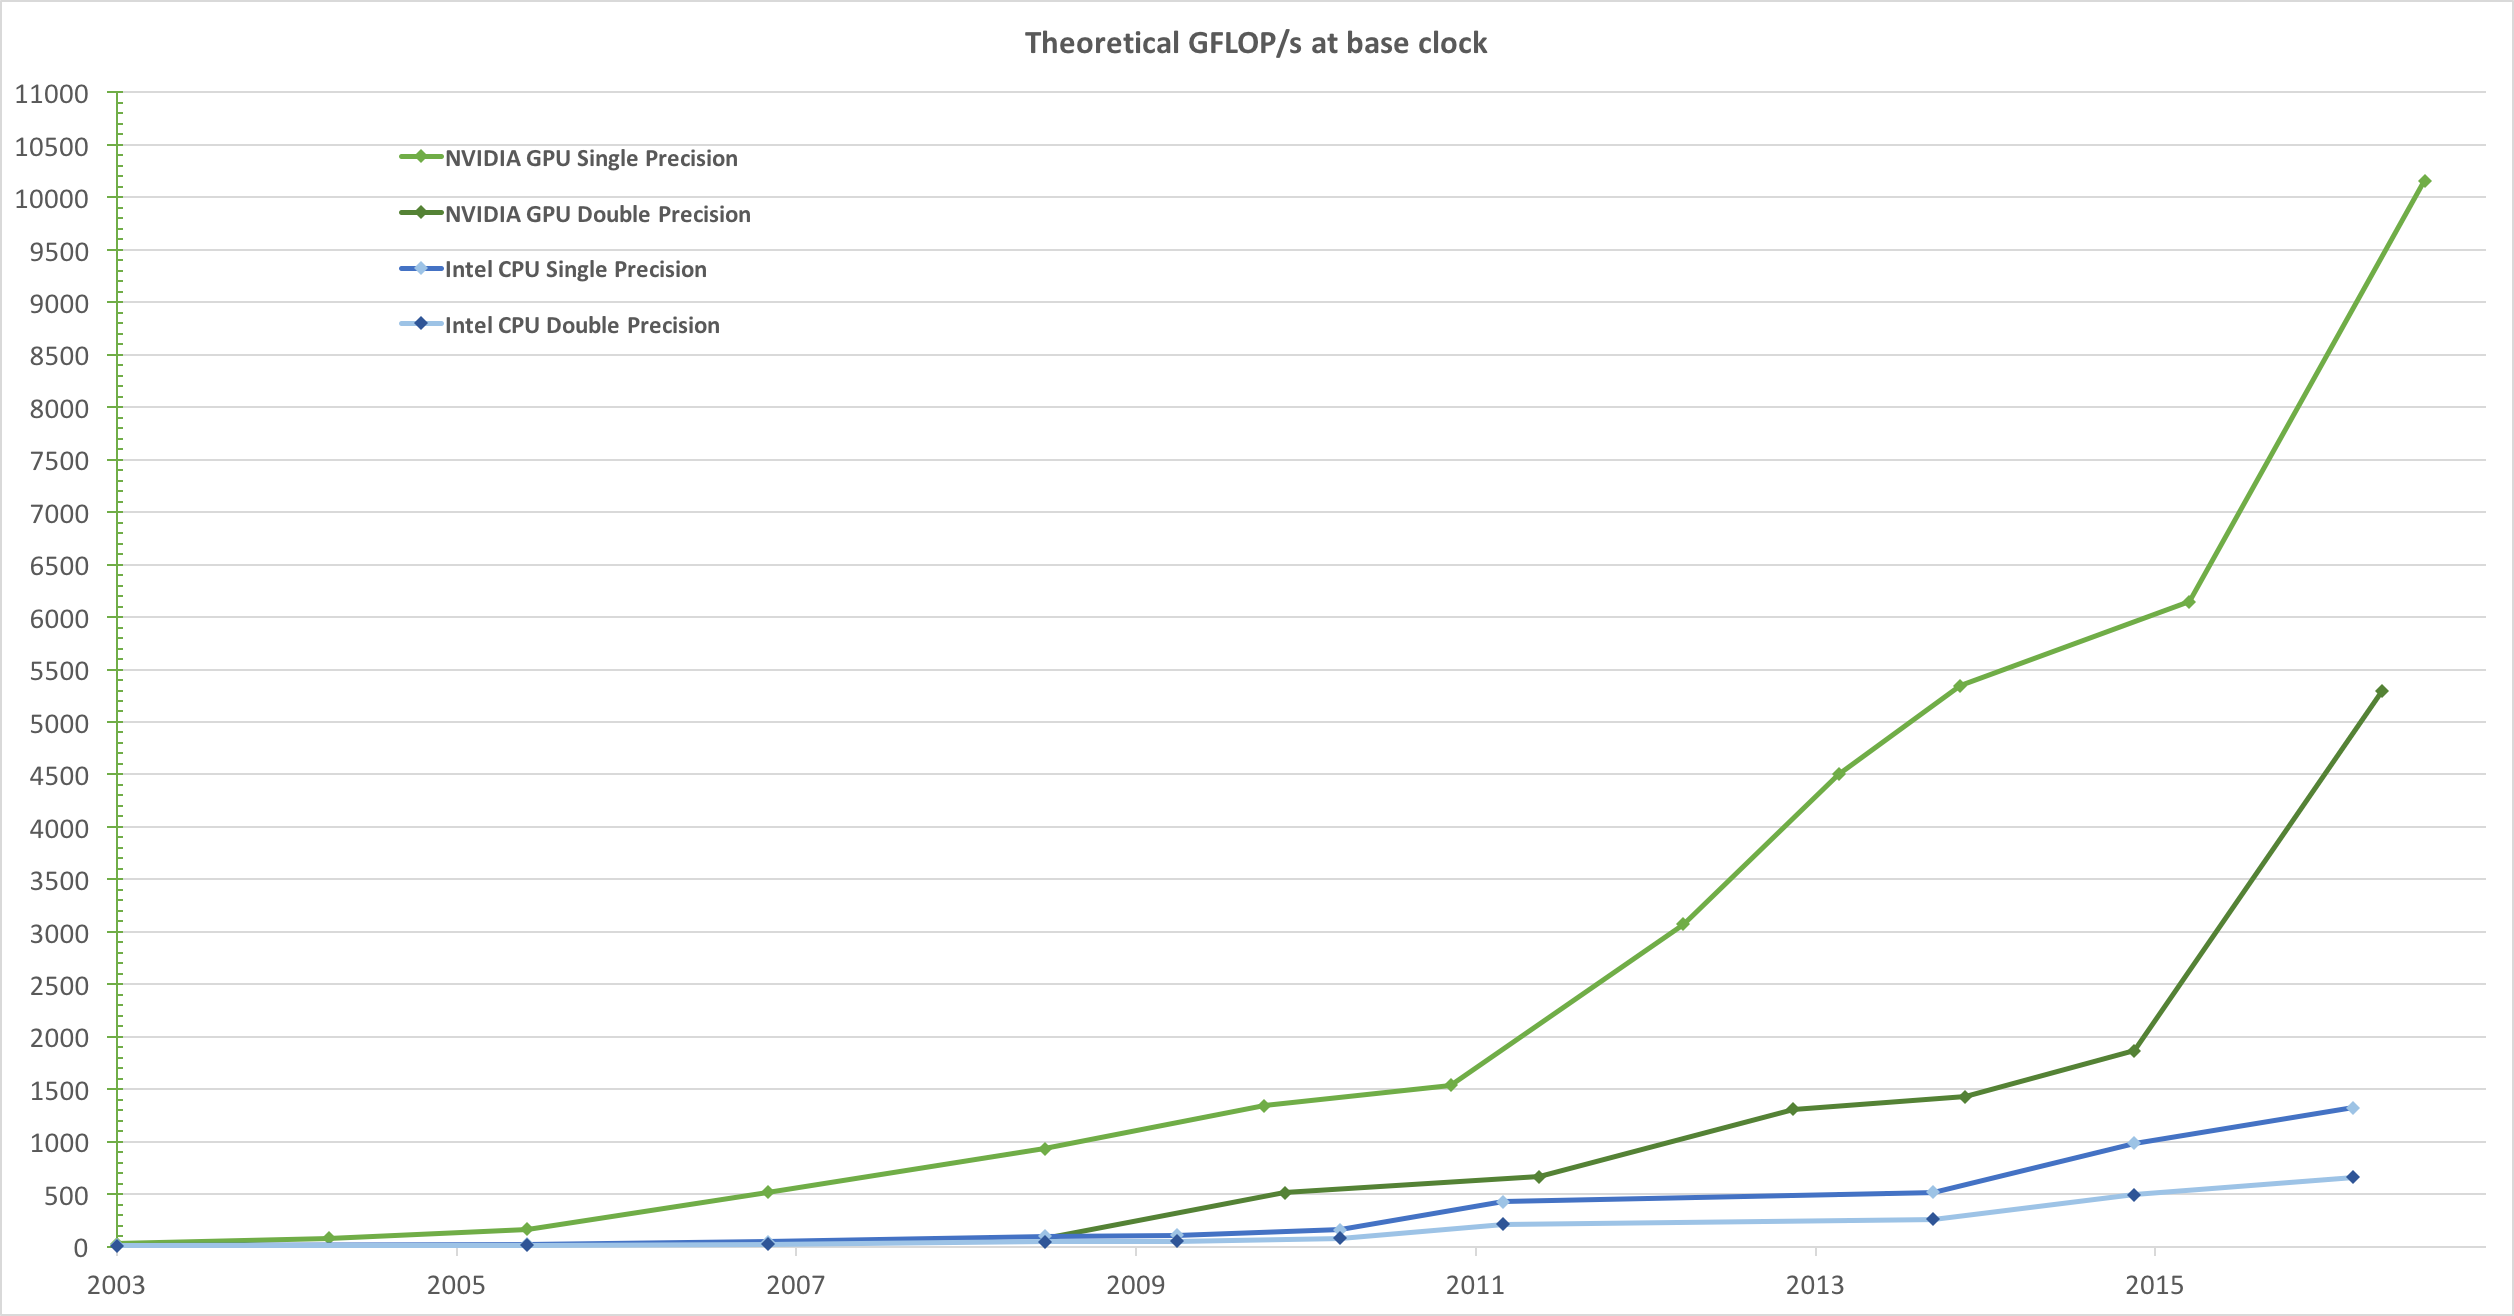
\includegraphics[width=1.0\textwidth]{gpu_comparison.png}
\end{frame}

\section{Concepts \& Methods}

\subsection*{CUDA}

\begin{frame}{CUDA}
	\begin{columns}[T]
		\begin{column}{0.75\textwidth}
			\begin{itemize}
				\item API for parallel computing on the GPU
				\item Developed by NVIDIA in 2007 
				\item Newest version: 8.0
				\item Support programming languages C/C++, Fortran, Python and many more
			\end{itemize}
		\end{column}
		\begin{column}{0.25\textwidth}
			
\includegraphics[width=1.0\textwidth]{cuda_logo.jpg}
		\end{column}
	\end{columns}
\end{frame}

\begin{frame}{Threads}
	\begin{columns}
		\begin{column}{0.45\textwidth}
			\centering 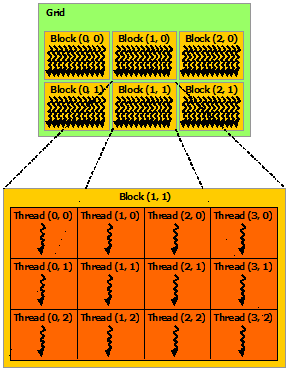
\includegraphics[width=0.9\textwidth]{cuda_threads.png}
		\end{column}
		\begin{column}{0.55\textwidth}
			\begin{itemize}
				\item Parallelization via "Device Kernels" with threads
				\item Organized in blocks on a grid
				\item Number of threads per block depends on architecture
				\item Blocks have access to shared memory
			\end{itemize}
		\end{column}
	\end{columns}
\end{frame}

\begin{frame}{Memory}
	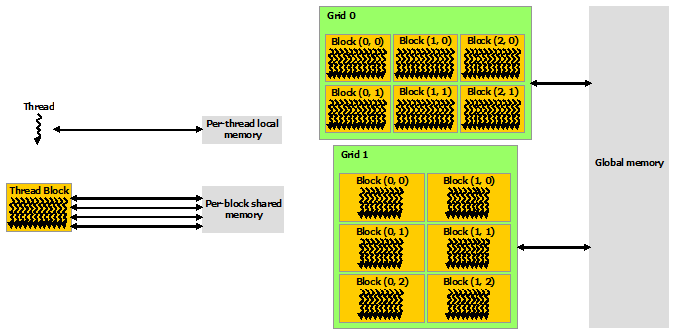
\includegraphics[width=1.0\textwidth]{cuda_memory.png}
\end{frame}

\begin{frame}{Example}
\end{frame}

\subsection*{k Nearest Neighbors}

\begin{frame}{Parallel kNN Search}
	\begin{columns}[T]
		\begin{column}{0.5\textwidth}
			\textbf{Naive Search}
			\begin{itemize}
				\item Highly parallelisable
				\item Low memory usage
				\item Quadratic runtime: $\mathcal{O}(n^2)$
				\item Asynchronous
			\end{itemize}
		\end{column}
		\begin{column}{0.5\textwidth}
			\textbf{kd-Tree}
			\begin{itemize}
				\item Only partial parallelisable
				\item Additional memory for tree representation necessary
				\item Approximately linear runtime: \mbox{$\mathcal{O}(n \cdot k \cdot \log(n))$}
				\item Synchronous
			\end{itemize}
		\end{column}
	\end{columns}
\end{frame}

\subsection*{Naive Search}

\begin{frame}{Basic Idea}
	\centering
	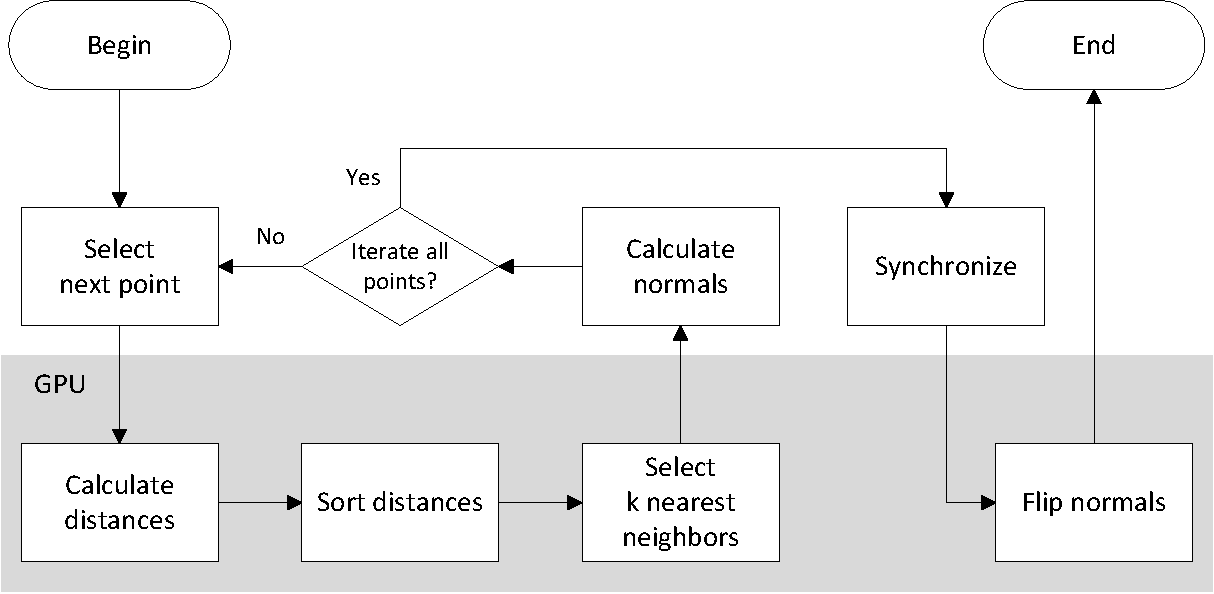
\includegraphics[width=0.9\textwidth]{knn_procedure.pdf}
\end{frame}

\begin{frame}{Implementation}
	\begin{algorithmic}
		\FORALL{points in data}
			\only<1>{\STATE calculate distances to all other points}
			\only<2>{\STATE \textcolor{red}{calculate distances to all other points}}
			\REPEAT
				\STATE count neighbors in radius of $\varepsilon$
				\STATE adapt $\varepsilon = \varepsilon \cdot (1 \pm \eta)$
			\UNTIL{number of neighbors in radius $\varepsilon = k$}
			\STATE get points in radius of $\varepsilon$
		\ENDFOR
	\end{algorithmic}
\end{frame}

\begin{frame}{Distance Calculation}
	\begin{columns}
		\begin{column}{0.5\textwidth}
			\begin{center}
				\only<1>{
				$\begin{pmatrix}
					6 & 0 & 1 & 6\\
					2 & 5 & 7 & 9\\
					4 & 5 & 9 & 4
				\end{pmatrix}$\\}
				\only<2->{
				$\begin{pmatrix}
					\textcolor{red}{6} & 0 & 1 & 6\\
					\textcolor{red}{2} & 5 & 7 & 9\\
					\textcolor{red}{4} & 5 & 9 & 4
				\end{pmatrix}$\\}
				\uncover<3->{$\Downarrow$\\
				$\begin{pmatrix*}[r]
					0 &  6 &  5 & 0\\
					0 & -3 & -5 & 7\\
					0 & -1 & -5 & 0
				\end{pmatrix*}$\\}
				\uncover<4>{$\Downarrow$\\
				$\begin{pmatrix}
					0 & 46 & 75 & 49
				\end{pmatrix}$}
			\end{center}
		\end{column}
		\begin{column}{0.5\textwidth}
			\begin{enumerate}
				\item \uncover<2->{Select point from matrix}
				\item \uncover<3->{Determine difference to each point dimension-wise}
				\item \uncover<4>{Calculate $d = x^2 + y^2 + z^2$}
			\end{enumerate}
		\end{column}
	\end{columns}
\end{frame}

\begin{frame}{Implementation}
	\begin{algorithmic}
		\FORALL{points in data}
			\STATE calculate distances to all other points
			\REPEAT
				\only<1>{\STATE count neighbors in radius of $\varepsilon$
				\STATE adapt $\varepsilon = \varepsilon \cdot (1 \pm \eta)$}
				\only<2>{\STATE \textcolor{red}{count neighbors in radius of $\varepsilon$}
				\STATE \textcolor{red}{adapt $\varepsilon = \varepsilon \cdot (1 \pm \eta)$}}
			\UNTIL{number of neighbors in radius $\varepsilon = k$}
			\STATE get points in radius of $\varepsilon$
		\ENDFOR
	\end{algorithmic}
\end{frame}

\begin{frame}{Distance 'Sorting'}
	\begin{columns}
		\begin{column}{0.5\textwidth}
			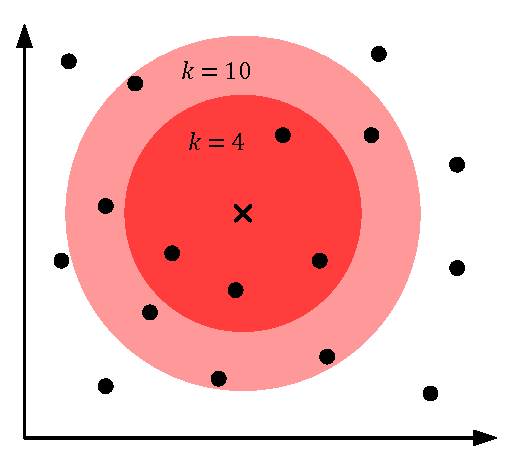
\includegraphics[width=1.0\textwidth]{radius_search.pdf}
		\end{column}
		\begin{column}{0.5\textwidth}
		\begin{itemize}
			\item Conventional sorting algorithms not applicable with parallel GPU computing
			\item Evaluate a distance $\varepsilon$ based on radius search
			\item Count $k$ inside radius $\varepsilon$
			\item Adapt $\varepsilon$ iteratively with learning rate $\eta$
		\end{itemize}
		\end{column}
	\end{columns}
\end{frame}

\subsection*{kd-Tree}

\begin{frame}{Basic Idea}
	\centering
	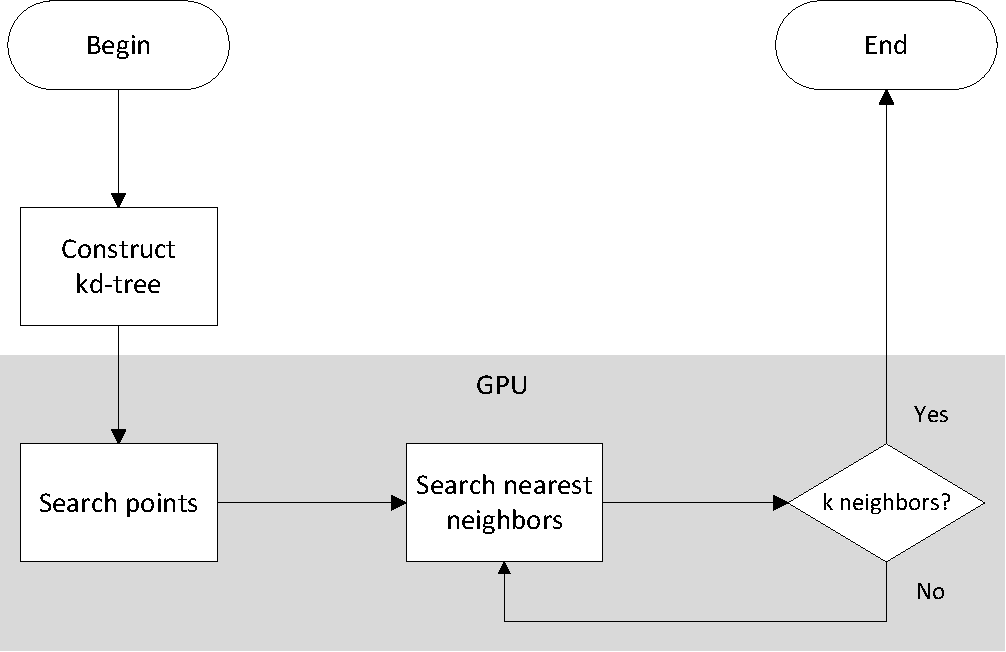
\includegraphics[width=0.9\textwidth]{kdtree_procedure.pdf}
\end{frame}

\begin{frame}{Tree Construction}
 	\centering
	\only<1>{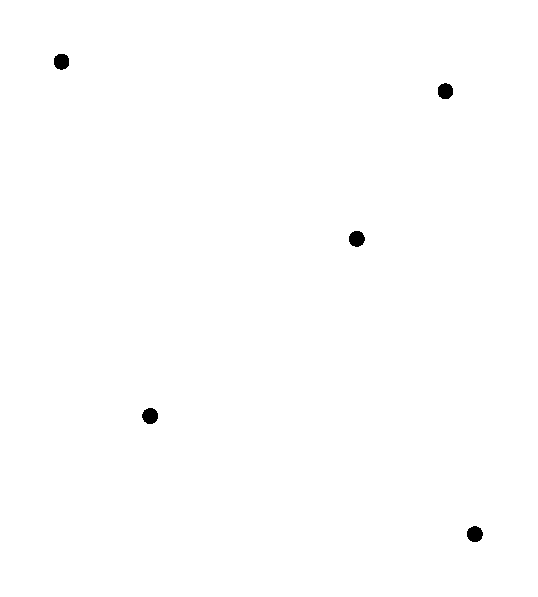
\includegraphics[width=0.5\textwidth]{kdtree_1.pdf}}
	\only<2>{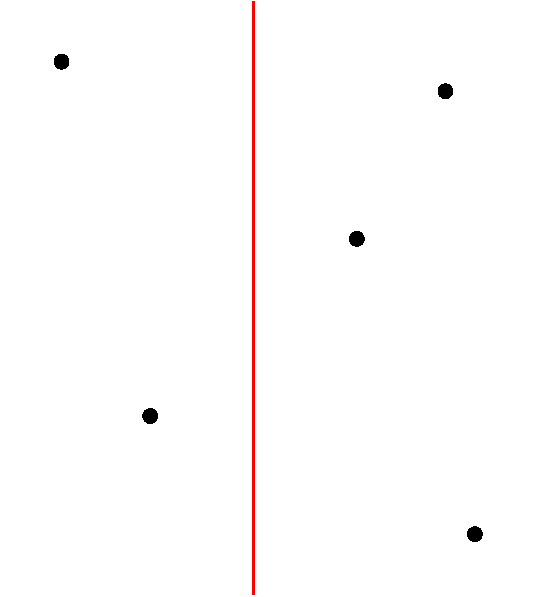
\includegraphics[width=0.5\textwidth]{kdtree_2.pdf}}
	\only<3>{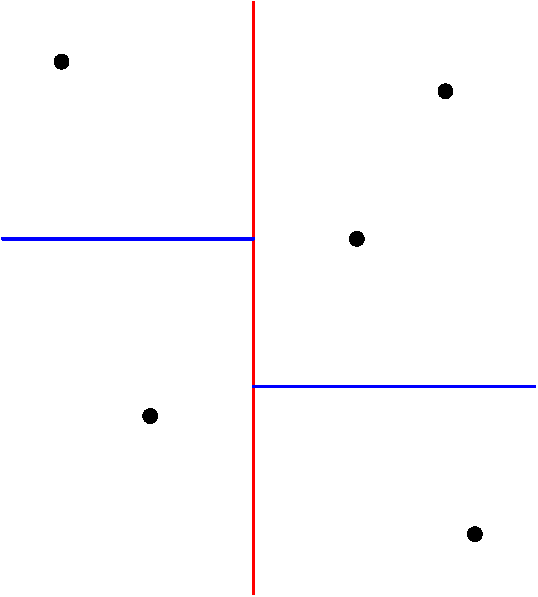
\includegraphics[width=0.5\textwidth]{kdtree_3.pdf}}
	\only<4>{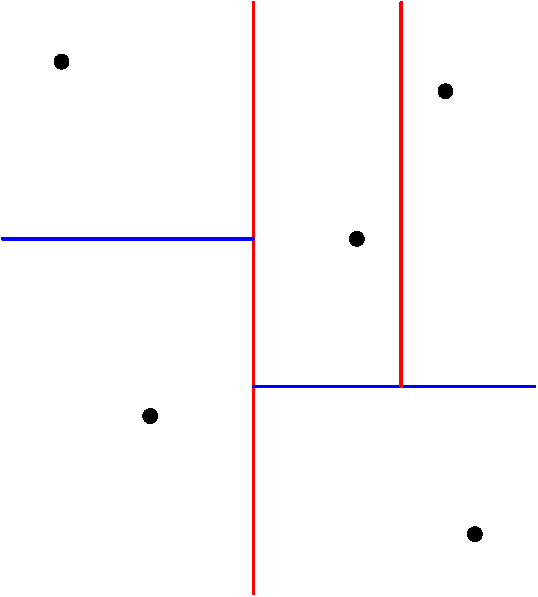
\includegraphics[width=0.5\textwidth]{kdtree_4.pdf}}
\end{frame}

\begin{frame}{Tree Construction}
	\begin{columns}
		\begin{column}{0.4\textwidth}
			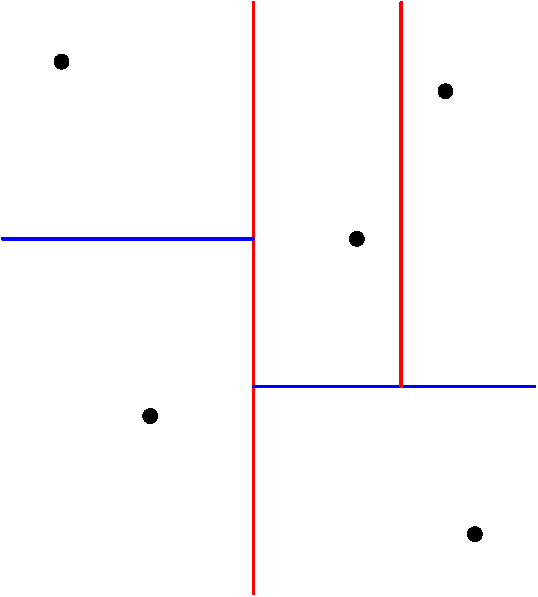
\includegraphics[width=1.0\textwidth]{kdtree_4.pdf}
		\end{column}
		\begin{column}{0.6\textwidth}
			\begin{itemize}
				\item Pre-partitioning of point cloud in the input space
				\item Average is between median and median $-\ 1$
				\item Generate recursively
				\item Construction time: $\mathcal{O}(n \cdot \log{n})$
				\item Memory usage: $2 \cdot n - 1 $
			\end{itemize}
		\end{column}
	\end{columns}
\end{frame}

\begin{frame}{Array-Based Left-Balanced kd-Tree}
	\centering
	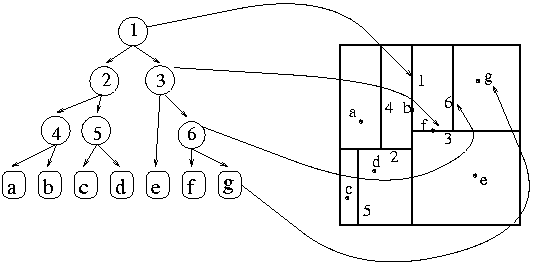
\includegraphics[width=0.9\textwidth]{kdtree.png}\\
	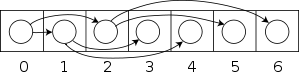
\includegraphics[width=0.5\textwidth]{kdtree_array.png}
\end{frame}

\begin{frame}{Array-Based Left-Balanced kd-Tree}
	\begin{columns}
		\begin{column}{0.5\textwidth}
			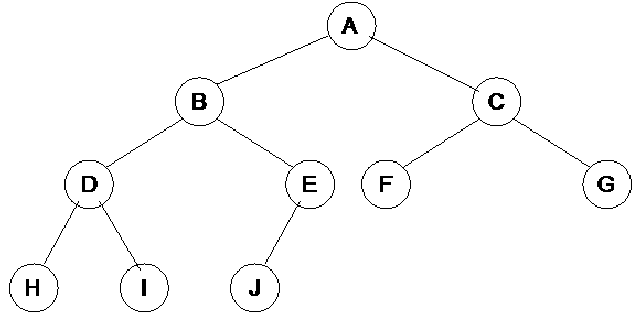
\includegraphics[width=1.1\textwidth]{left_balanced_tree.png}
		\end{column}
		\begin{column}{0.5\textwidth}
			\begin{itemize}
			\item Required space
				\begin{itemize}
					\item Array median: \mbox{$S = \min{2^i}$ s.t. $S \geq 2n - 1$}
					\item Array left-balanced: $S = 2n - 1$
				\end{itemize}
				\item Left-balanced split is fast computable
			\end{itemize}
		\end{column}
	\end{columns}
\end{frame}

\begin{frame}{Split Rule}
	\begin{algorithmic}
		
		\STATE calculate $ 2^{x} = N-1 $ 
		\STATE $pot \gets \lfloor x \rfloor $
		\STATE $right \gets 2^{pot-1} $
		\STATE $left \gets (N - r)$
		\STATE $v \gets 2^{pot} $
		\IF { $ left > v $ }
			\STATE $ right \gets right + left - v $
			\STATE $ left \gets v $
		\ENDIF
		
	\end{algorithmic}
\end{frame}



\begin{frame}{GPU}
	\begin{itemize}
		\item Allocate memory on device for 
		\begin{itemize}
			\item Point cloud: $ N*3 $
			\item kd-Tree: $ (2N-1) $
			\item Normals:$ N*3 $
			\item Total: $ N*8 - 1 $
		\end{itemize}
		\item Copy point cloud, kd-Tree to device
		\item Start GPU-Kernel
		\begin{itemize}
			\item Get maximum number of threads
			\item Calculate number of blocks
		\end{itemize}
	\end{itemize}
\end{frame}

\begin{frame}{kd-Tree Search}
	\begin{algorithmic}
		\STATE $ q \gets Querypoint , dim \gets 0, pos \gets root$
		\WHILE { $ pos \cdot 2 + 1 < kdtree.size $ }
			\STATE $ s \gets kdtree.split $
			\IF{ $ q[dim] < s $ }
				\STATE $ pos \gets pos \cdot 2 + 1 $
			\ELSE
				\STATE $ pos \gets pos \cdot 2 + 2 $
			\ENDIF
			\STATE $ dim \gets (dim+1)\%3 $
		\ENDWHILE
	\end{algorithmic}
\end{frame}

\begin{frame}{kd-Tree KNN}
	\centering
	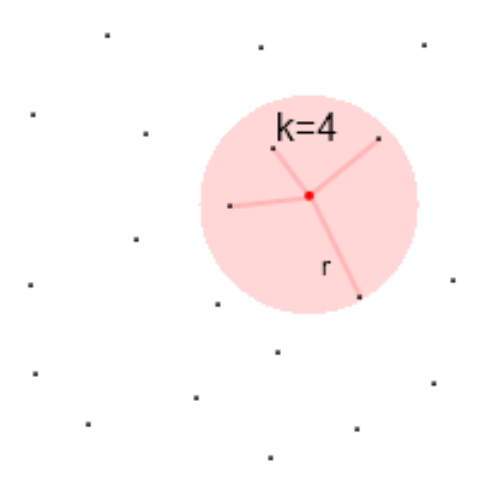
\includegraphics[height=0.7\textheight]{knn.png}
\end{frame}

\begin{frame}{kd-Tree KNN}
	\small
	\begin{algorithmic}
		\STATE define nn as a set of nearest neighbors
		\STATE initialize radius with 0
		\WHILE { size of nn < k }
			\STATE add parents other subtree leafs to nn
			\STATE update radius to the max found distance
			\STATE go up
		\ENDWHILE
		
	\end{algorithmic}
\end{frame}

\begin{frame}{kd-Tree KNN}
	\small
	\begin{algorithmic}
		\WHILE{ distance of query point three upper tree nodes < radius }
			\STATE go up
			\STATE check neighbor cell for shorter distances
			\FOR {points with shorter distances}
				 \STATE update nn
				 \STATE update radius
			\ENDFOR
		\ENDWHILE
	 
	\end{algorithmic}

\end{frame}

\begin{frame}{kd-Tree KNN}
\centering
	\only<1>{
		k=2  \\
		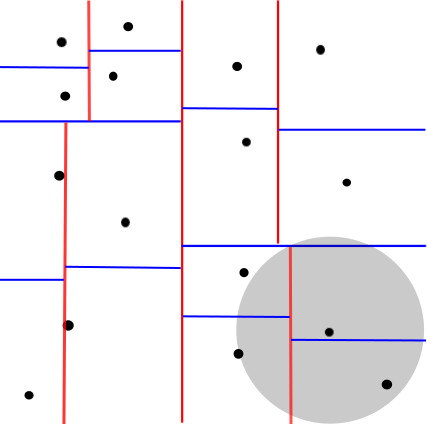
\includegraphics[height=0.7\textheight]{knn1.png}
	}
	\only<2>{
		k=2 \\
		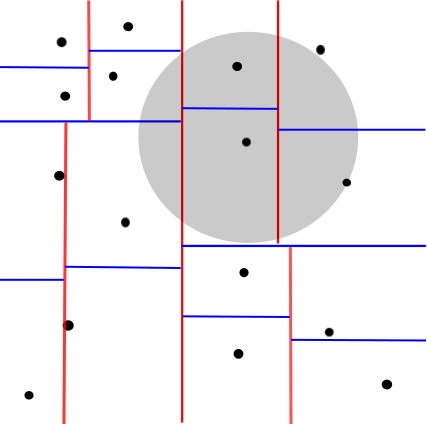
\includegraphics[height=0.7\textheight]{knn2.png}
	}
\end{frame}

\subsection*{Normal Calculation}

\begin{frame}{Normal Calculation}
	\centering
	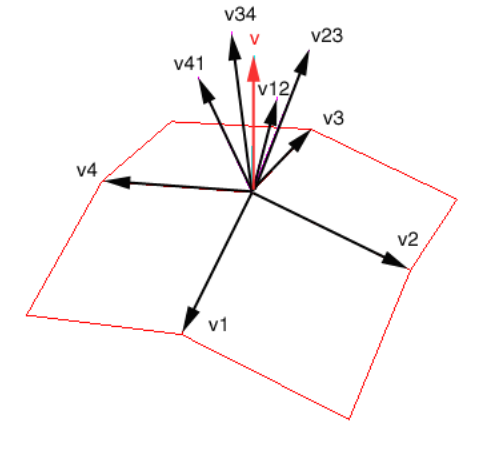
\includegraphics[width=0.6\textwidth]{normal_calculation.png}
\end{frame}

\begin{frame}{Normal Calculation}
	\begin{columns}
		\begin{column}{0.4\textwidth}
			\centering
			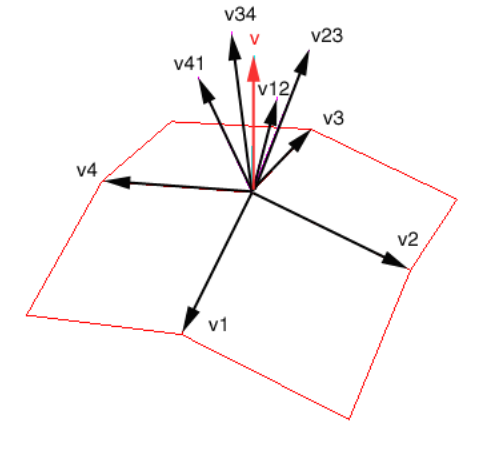
\includegraphics[width=1.0\textwidth]{normal_calculation.png}
		\end{column}
		\begin{column}{0.6\textwidth}
			\begin{itemize}
				\item Find best normal of the given set
				\item Distance point to plane: $d(p,n) = |\langle p,n \rangle|$
				\item Error: $E(n_i) = \sum\limits^{p}{d(p,n_i)}$
				\item Minimize $E$ to achieve best normal
				\item Speed-up: interrupt when error $E$ converges
			\end{itemize}
		\end{column}
	\end{columns}
\end{frame}

\begin{frame}{Normal Flip}
	\begin{columns}
		\begin{column}{0.5\textwidth}
 			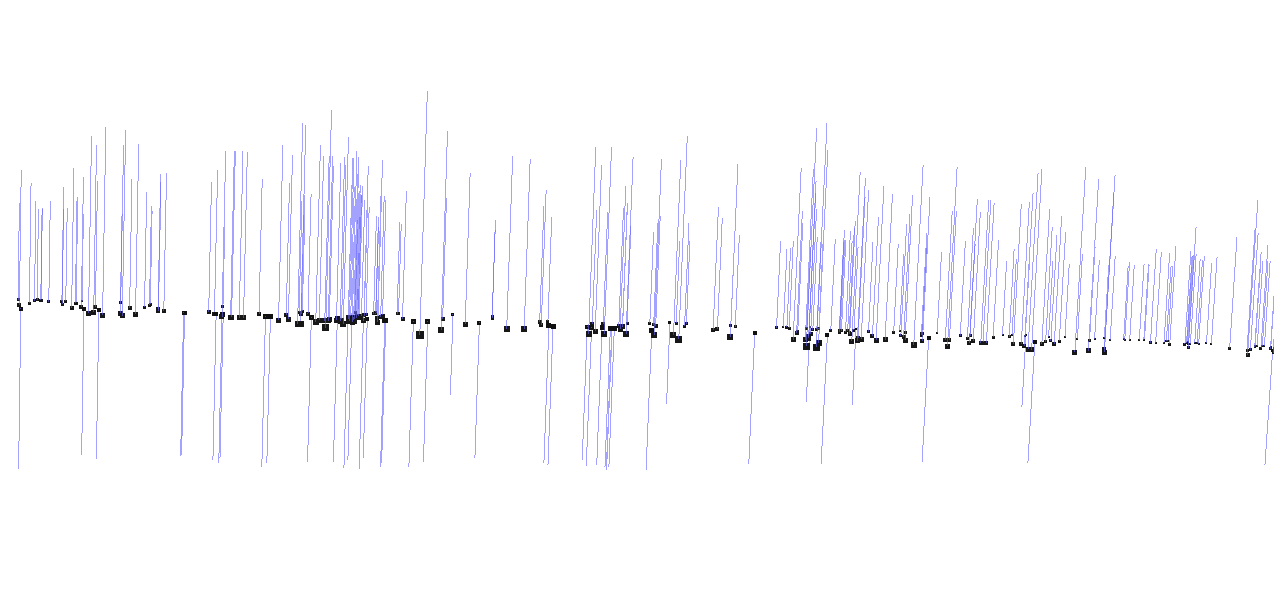
\includegraphics[width=1.0\textwidth]{normal_flip.png}\\
			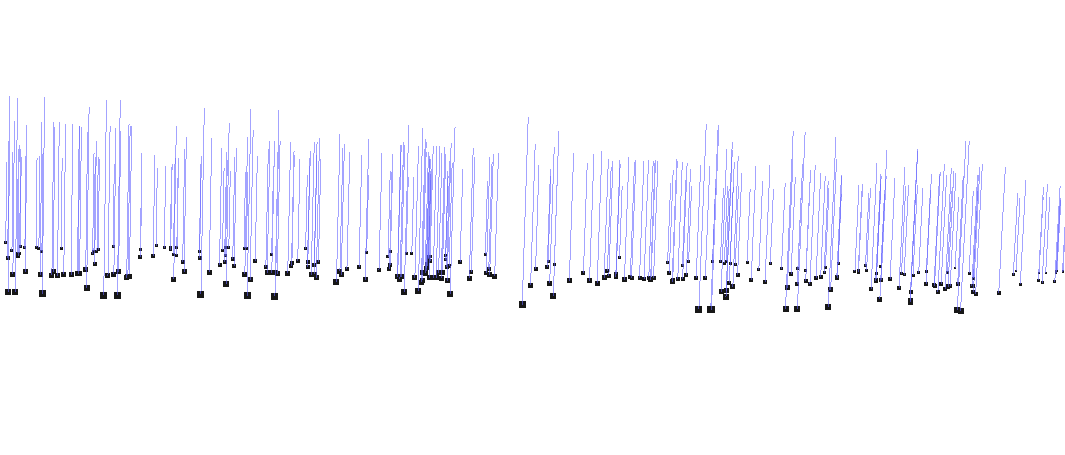
\includegraphics[width=1.0\textwidth]{normals.png}
		\end{column}
		\begin{column}{0.5\textwidth}
			\begin{itemize}
				\item Flip normals to view point $v$
				\item If $\langle n,v \rangle < 0$ then flip! 
				\item Flip: $n = -n$
			\end{itemize}
		\end{column}
	\end{columns}
\end{frame}

\section{Results}

\subsection*{Runtime}

\begin{frame}{Experiment Setting}
	\begin{itemize}
		\item Runtime comparison
		\begin{itemize}
			\item CUDA naive search (GeForce GTX 745, 4GB)
			\item CUDA kd-tree (GeForce GTX 745, 4GB)
		\end{itemize}
		\item One model of a real-world point cloud
		\item Reduced to specific number of points $n$
		\item Maximum $n$: $1\,000\,000$
		\item Step size: $50\,000$
	\end{itemize}
\end{frame}

\begin{frame}{Naive Search vs. kd-Tree}
	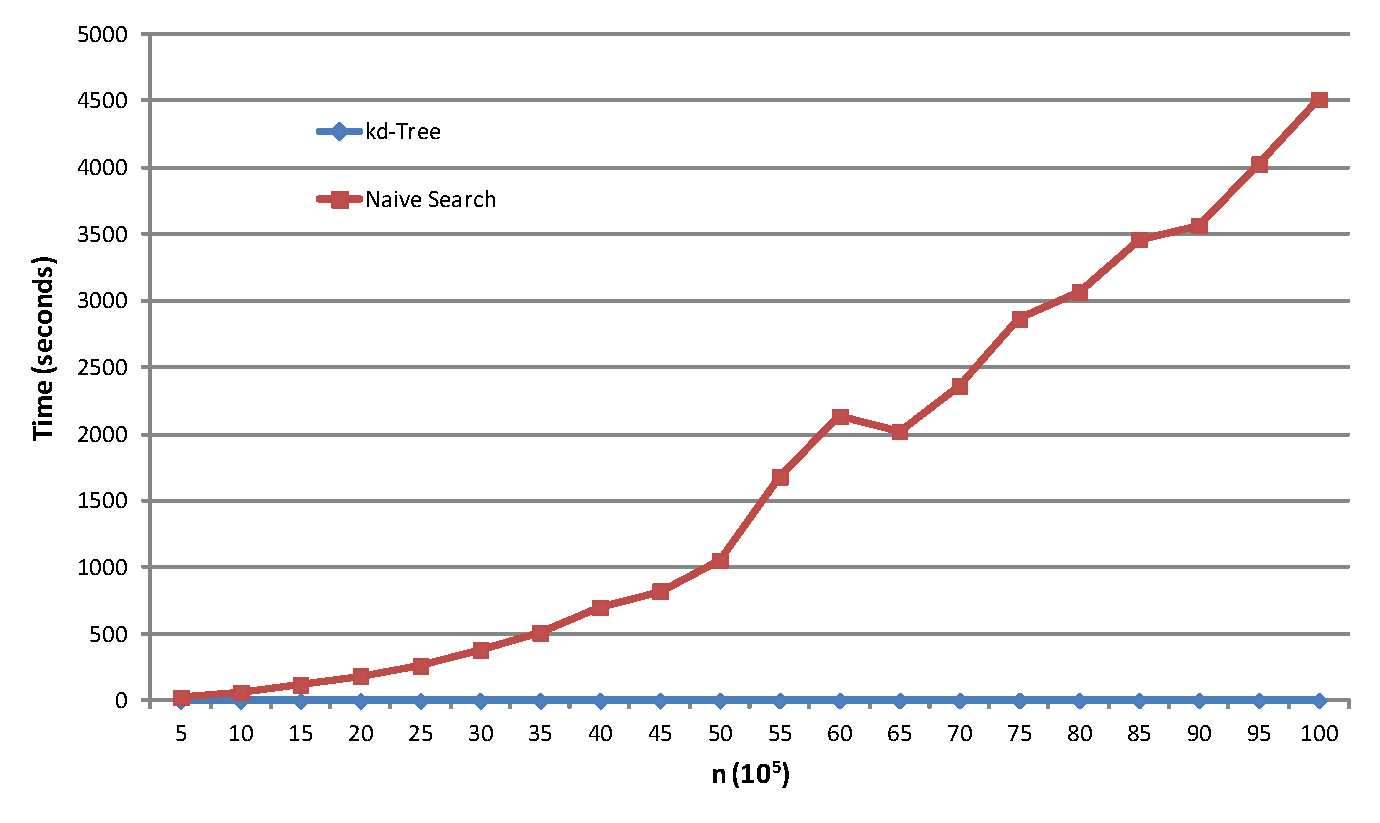
\includegraphics[width=1.0\textwidth]{plot_1.pdf}
\end{frame}

\begin{frame}{Experiment Setting}
	\begin{itemize}
		\item Runtime comparison
		\begin{itemize}
			\item CUDA kd-tree (GeForce GTX 745, 4GB)
			\item CPU multi-threaded kd-tree from LVR \mbox{(i7-4710HQ, 2.50 GHz, 8 Threads)}
		\end{itemize}
		\item One model of a real-world point cloud
		\item Reduced to specific number of points $n$
		\item Maximum $n$: $20\,000\,000$
		\item Step size: $1\,000\,000$
	\end{itemize}
\end{frame}

\begin{frame}{GPU kd-Tree vs. CPU kd-Tree LVR}
	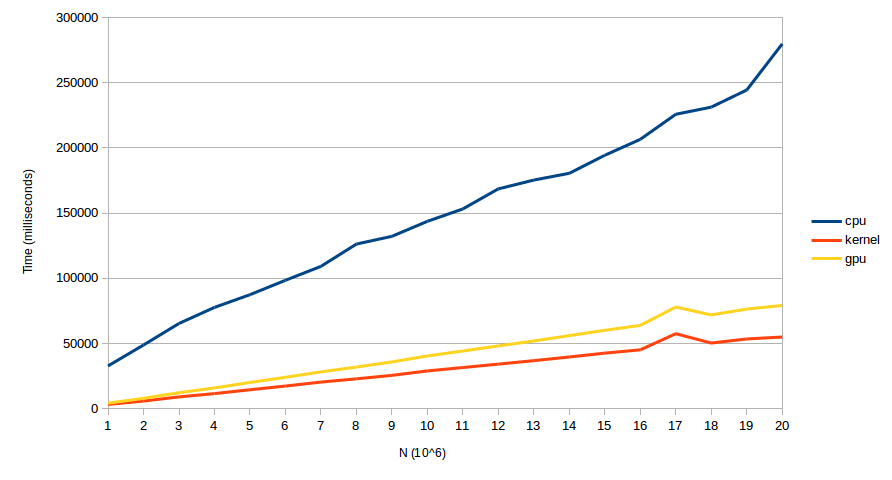
\includegraphics[width=1.0\textwidth]{cpu_gpu_results.png}
\end{frame}

\subsection*{LVR Pipeline}

\begin{frame}{Normals}
 	\begin{figure}
  		\centering
  		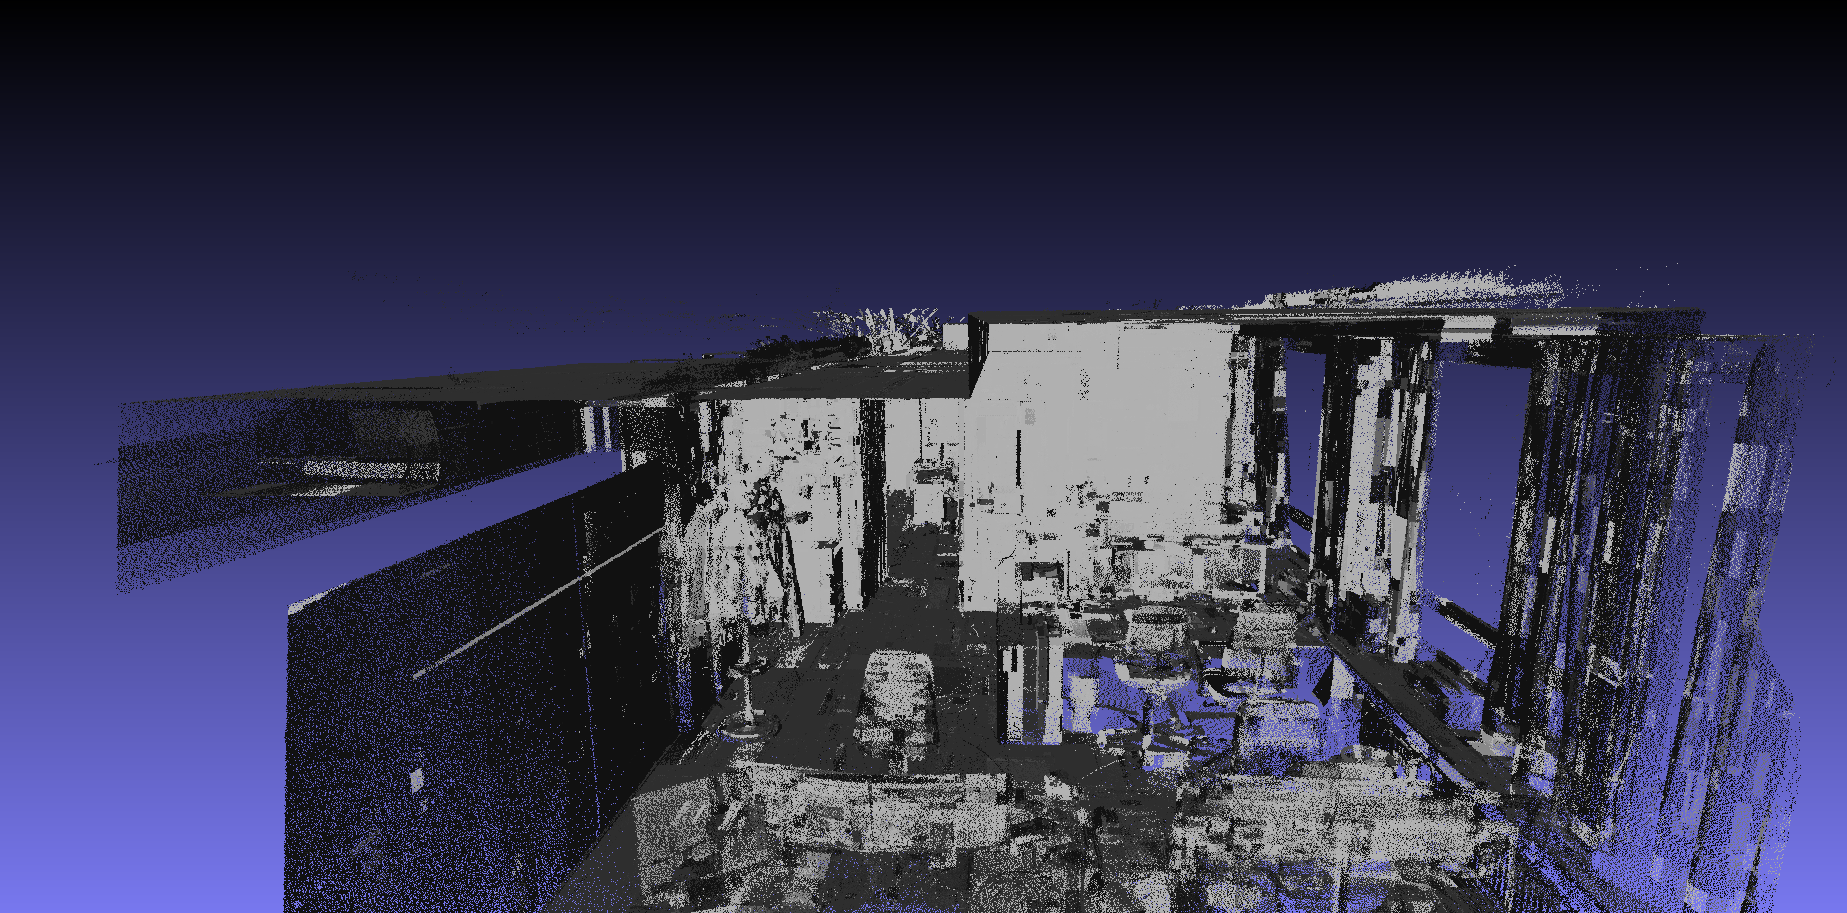
\includegraphics[height=0.39\textheight]{police_no_normals.png}\\
  		\vspace{0.1cm}
  		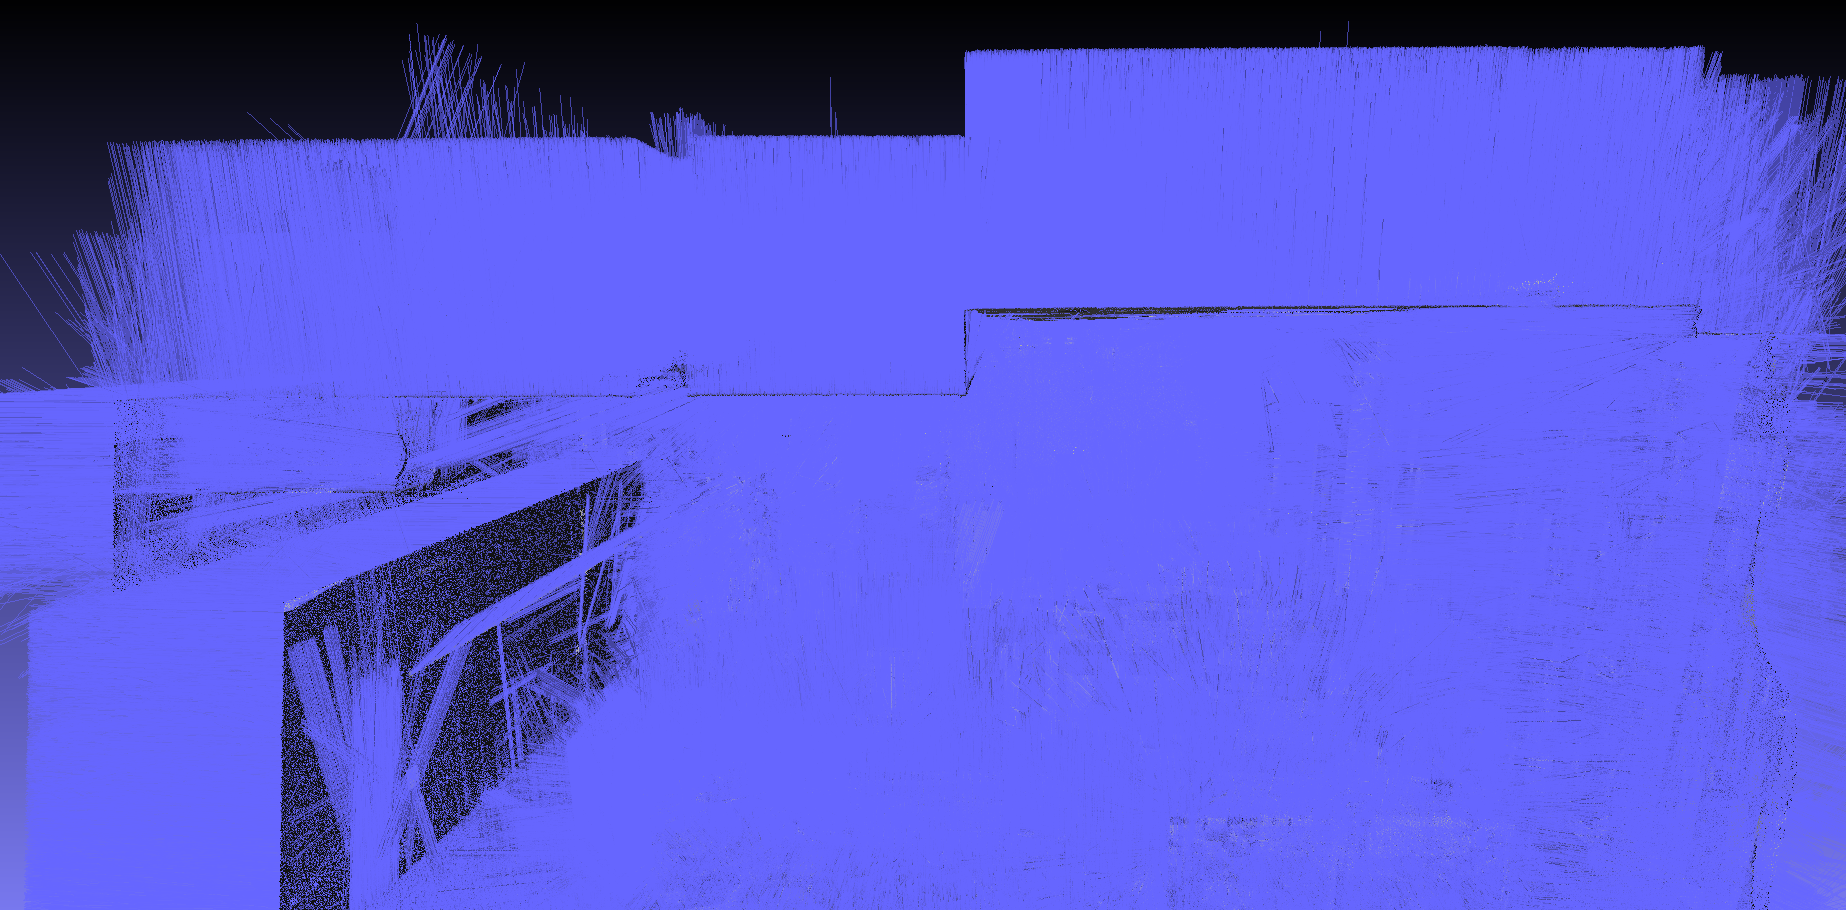
\includegraphics[height=0.39\textheight]{police_normals.png}
	\end{figure}
\end{frame}

\begin{frame}{Normals}
	\begin{figure}
   		\centering
   		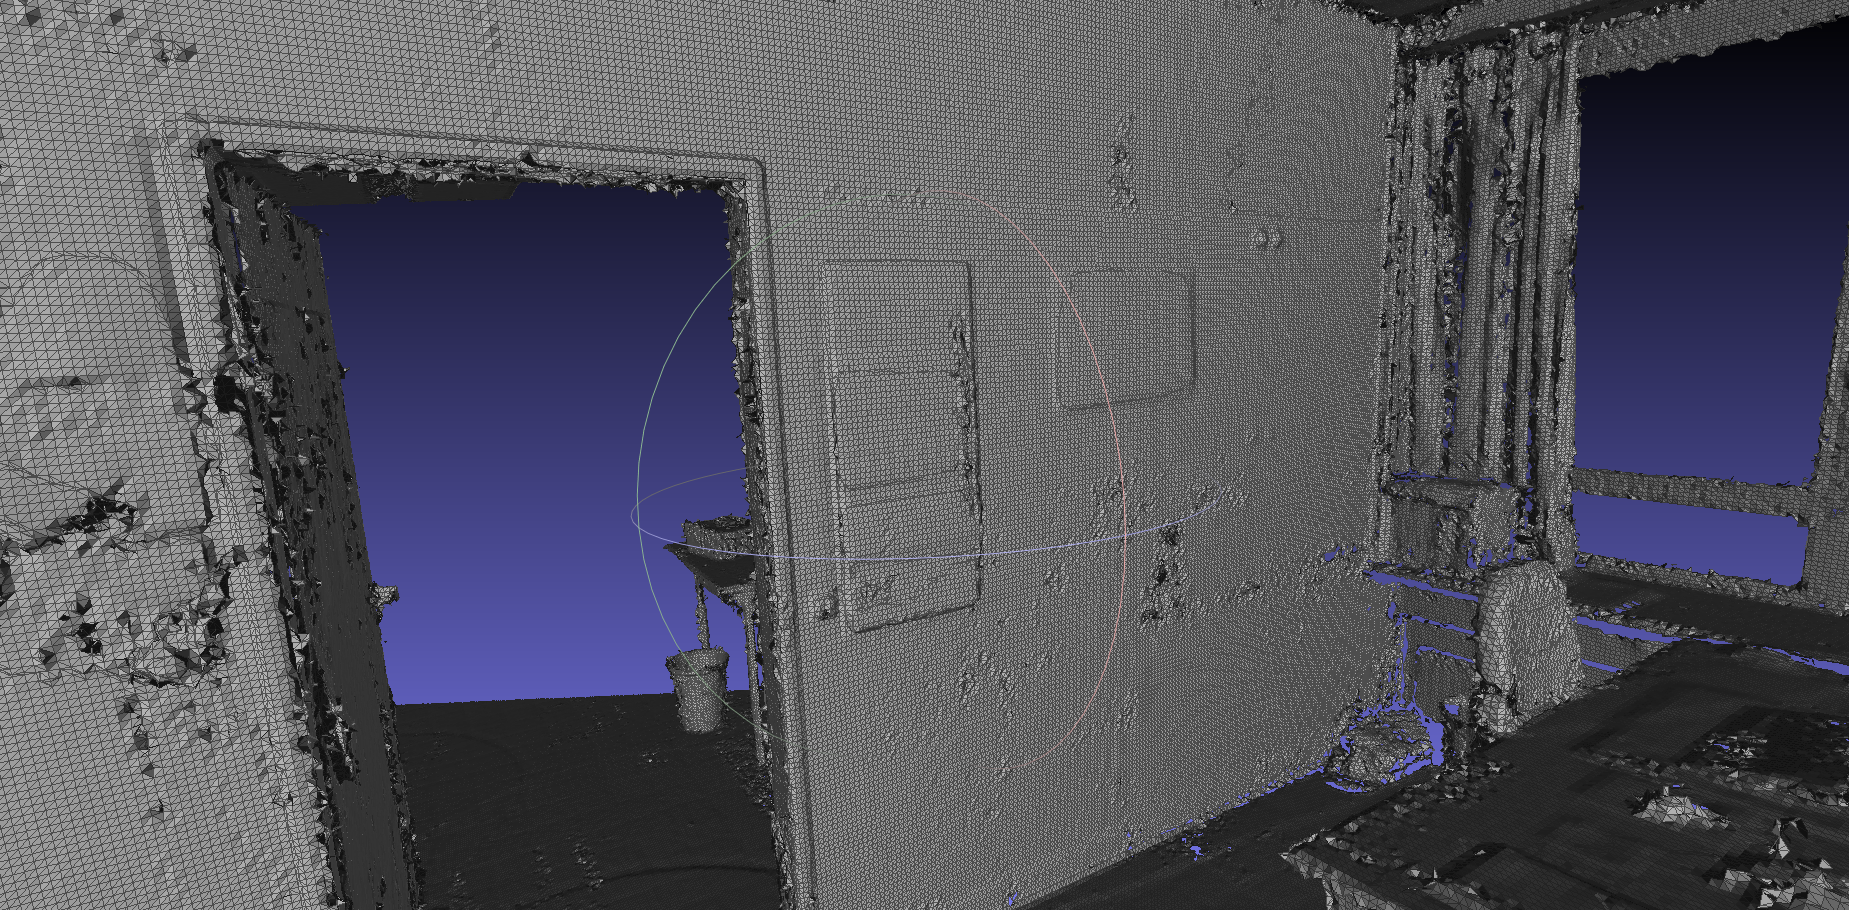
\includegraphics[height=0.39\textheight]{police_mesh.png}\\
   		\vspace{0.1cm}
   		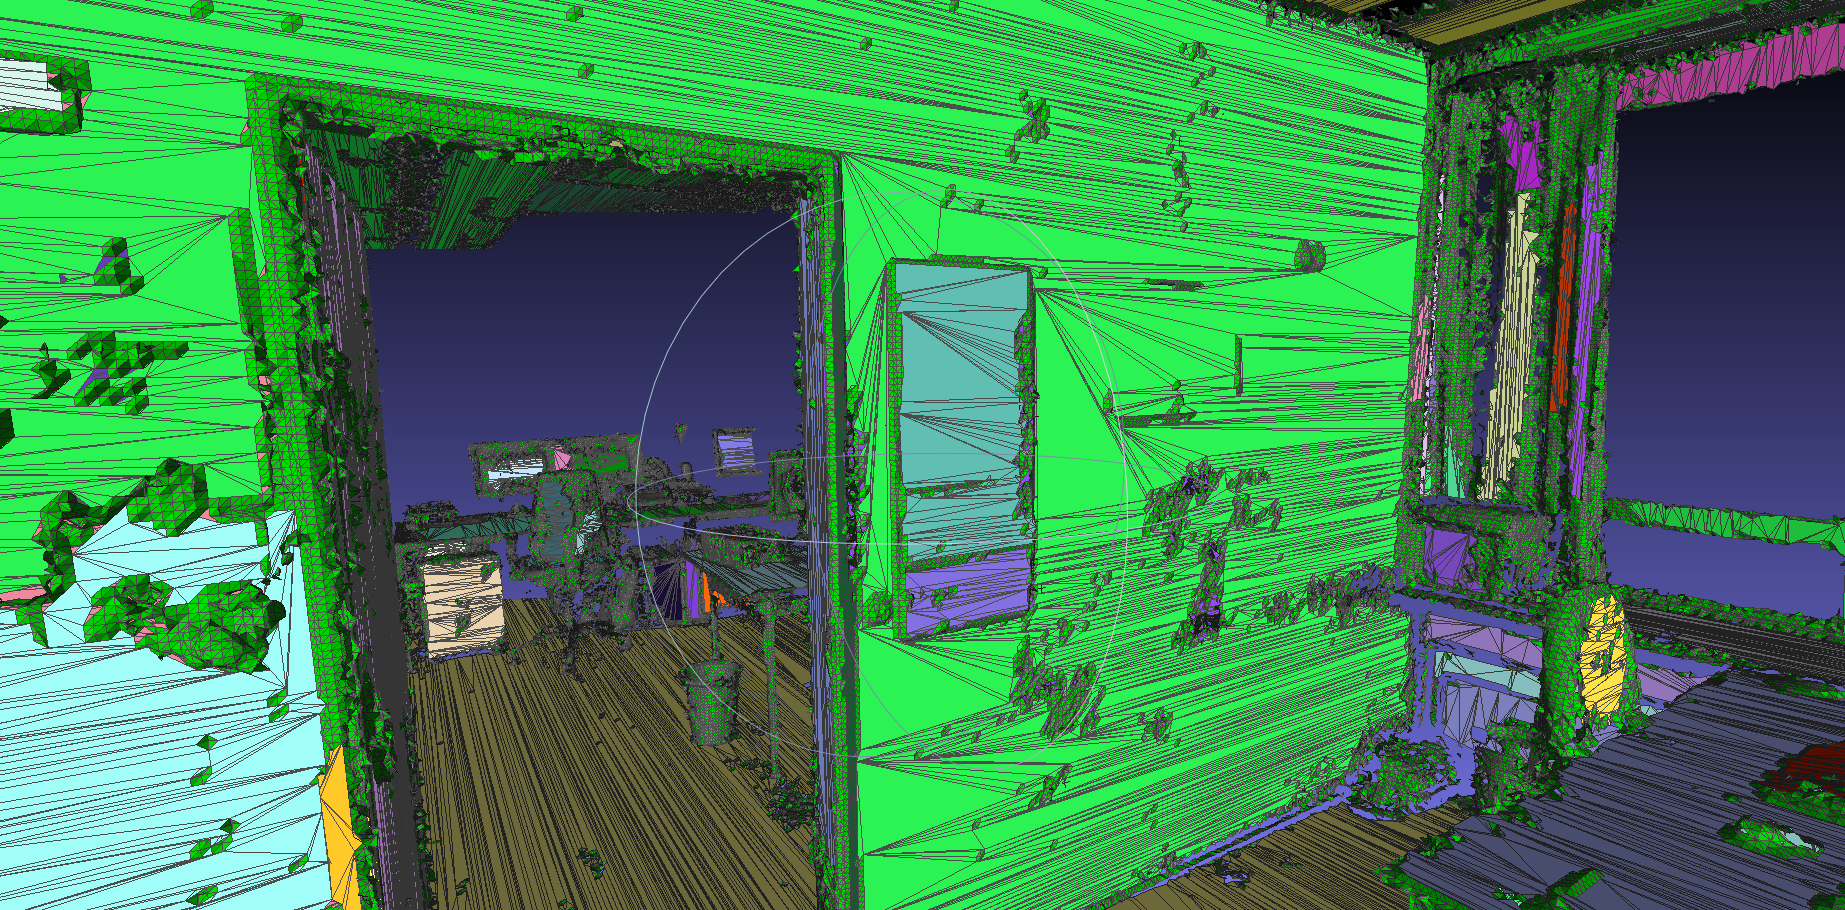
\includegraphics[height=0.39\textheight]{police_opt_mesh.png}
  	\end{figure}
\end{frame}

\begin{frame}{Discussion}
\end{frame}

\section{Conclusion}

\begin{frame}{Conclusion}
\end{frame}

\end{document}
